

\subsubsection*{Scenario: Quadratic}
Next we consider two-degree polynomials, which contain only quadratic terms. They take the form: $$g_2(x_1, x_2) = a_{11} x_1^2 + a_{22} x_2^2.$$
From \autoref{eq:fanova_components_2D_polynomial} we can derive the fANOVA components for $g_2$:
\begin{align*}
    y_{\emptyset} &= a_{11} + a_{22}, \\
    y_1(x_1) &= a_{11}(x_1^2 - 1), \\
    y_2(x_2) &= a_{22}(x_2^2 - 1).
\end{align*}
In \autoref{fig:quadratic_main_effects}, we vary the coefficients $a_{11}$ and $a_{22}$, while the interaction term is again absent.
Here we deal with two parabolas for the main effect and know that the sign of the coefficients determines their direction, while the magnitudes influence how stretched or compressed they are. The constant fANOVA component $y_{\emptyset}$ is present here, but as it only shifts the decomposition along the y-axis, it does not affect the form of the effect functions, therefore we do not visualize it.

\begin{figure}[htpb]
    \centering
    \begin{subfigure}[t]{0.49\textwidth}
        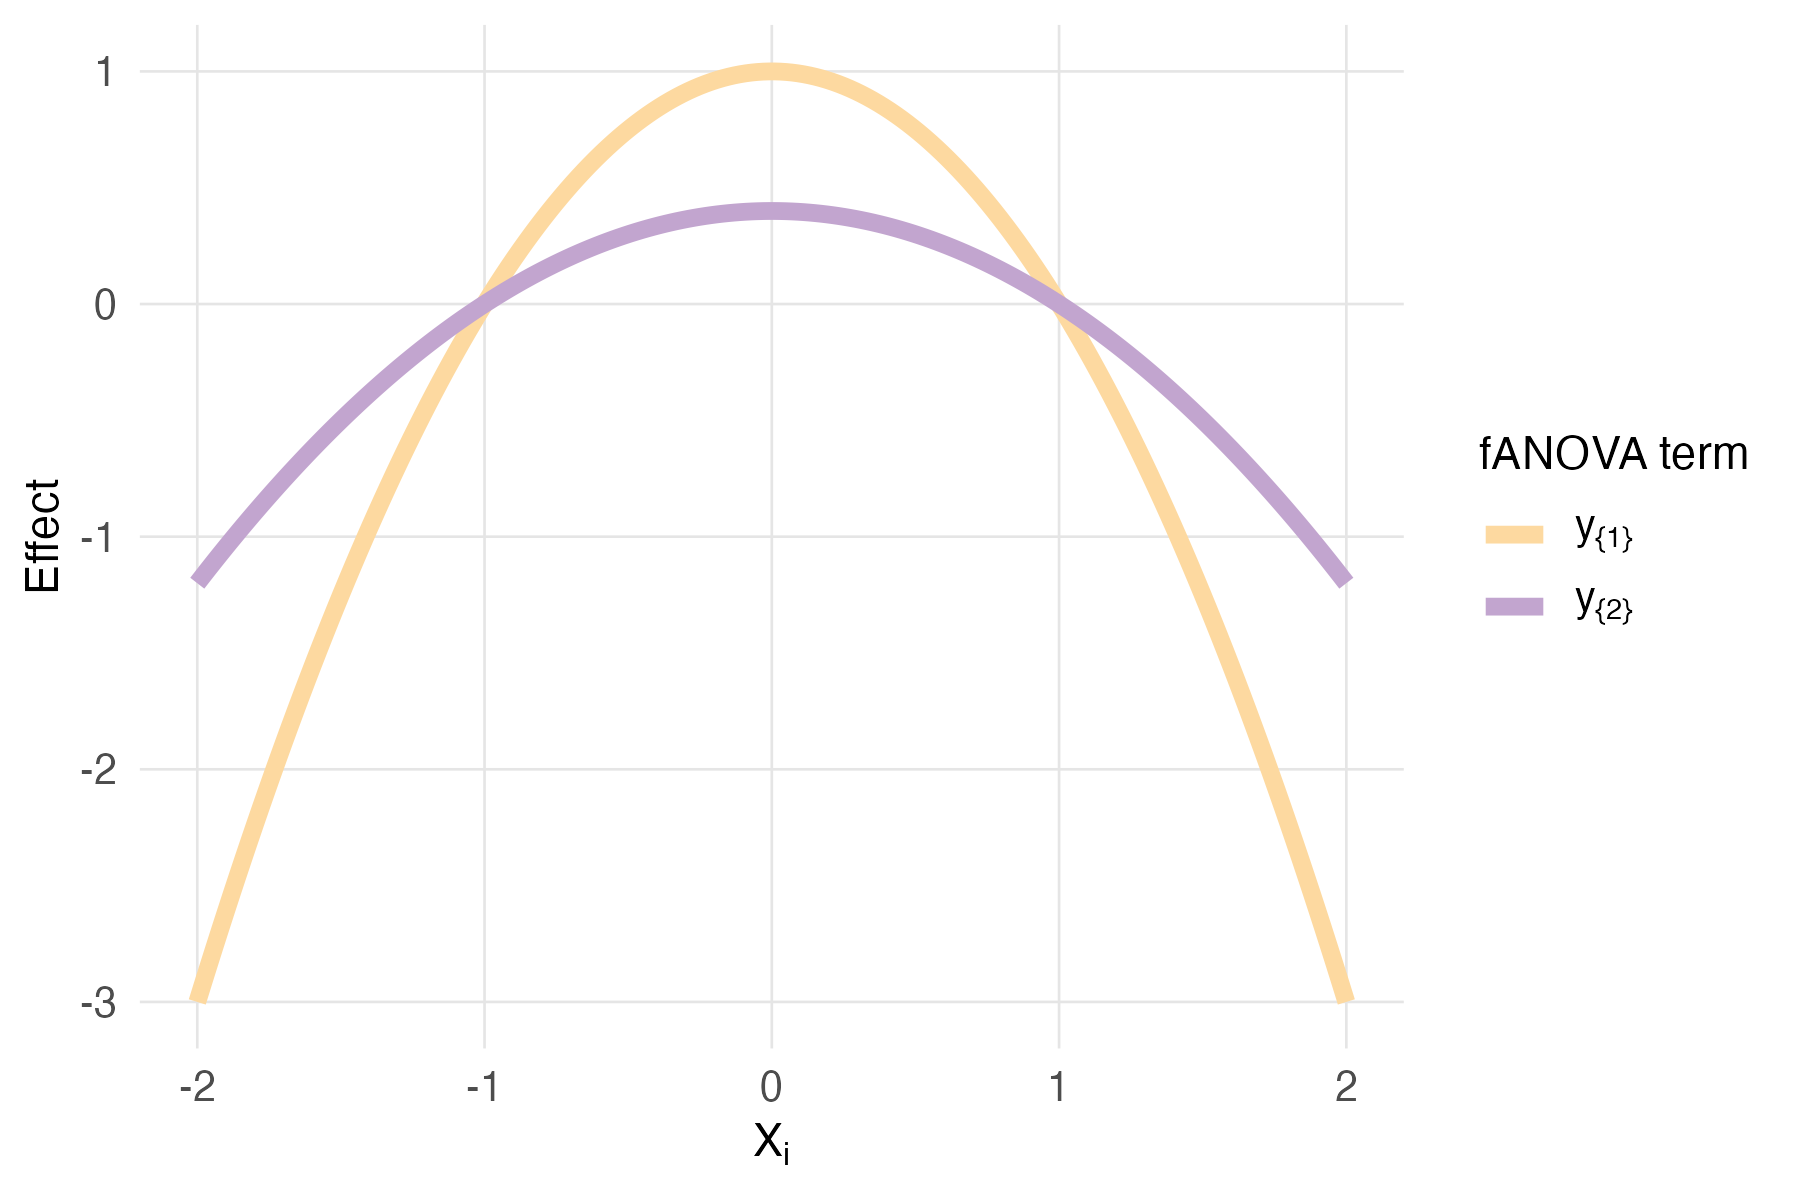
\includegraphics[width=\textwidth]{images/experiment_section/quadratic_a1p00_a2p00_a11m10_a22m04_a12p00_rhop00_main.png}
        \caption{$a_{11} = -1$, $a_{22} = -0.4$}
    \end{subfigure}%
    \hfill
    \begin{subfigure}[t]{0.49\textwidth}
        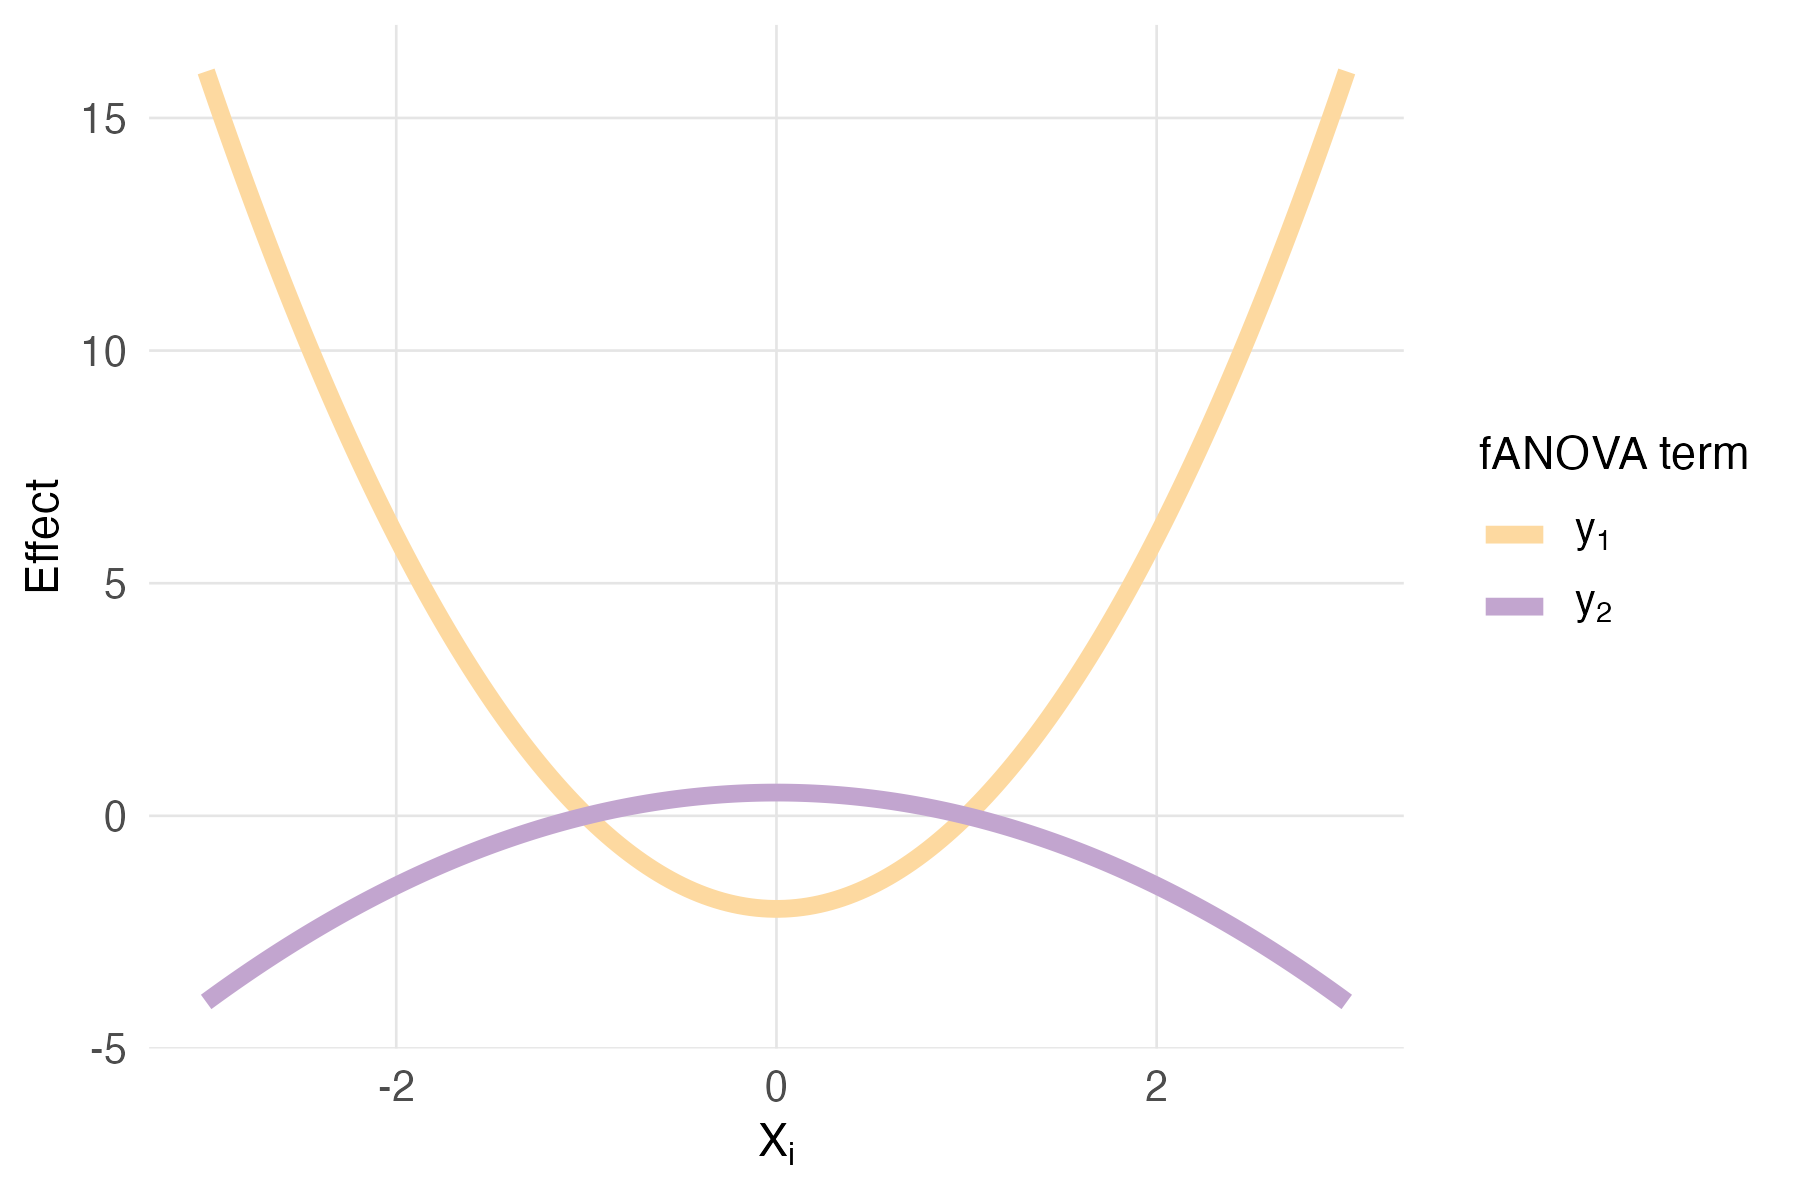
\includegraphics[width=\textwidth]{images/experiment_section/quadratic_a1p00_a2p00_a11p20_a22m05_a12p00_rhop00_main.png}
        \caption{$a_{11} = 2$, $a_{22} = -0.5$}
    \end{subfigure}
    \caption{Main effects for quadratic terms with different coefficients. The fANOVA components are given by: $y_1(x_1) = a_{11}(x_1^2 - 1)$, $y_2(x_2) = a_{22}(x_2^2 - 1)$.}
    \label{fig:quadratic_main_effects}
\end{figure}

\subsubsection*{Analytical Example Functions for fANOVA}

We present a selection of analytically tractable functions that highlight different behaviors of the fANOVA decomposition.

\paragraph{Sparse additive + interaction (low effective dimensionality).}
These functions illustrate cases where only a few variables or low-order interactions dominate the variance, allowing fANOVA to compress the functional complexity:
\[
f_1(x) = x_1 + x_2 \cdot x_3
\]


\paragraph{Smooth localized function.}
This function is smooth but has variance concentrated in a small region of the input space. It can be used to explore how fANOVA captures global variance, not localized effects:
\[
f_3(x, y) = \exp\left(-100(x^2 + y^2)\right)
\]
Each of these functions can be used to stress-test specific characteristics of the fANOVA decomposition: sparsity, interaction order, locality, and smoothness.

\section{Further examples}


\paragraph{Identifying interaction clusters}
This example shows that all the cross-terms vanish. So fANOVA correctly identifies that we have interaction pairs and no term is appearing multiple times in two or more interaction groups.
\begin{align*}
f(x) &= (x_1 + x_2)^2 + x_3 x_4 + \sin(x_5 x_6) \\[1em]
y_\emptyset &= \mathbb{E}[f] = \mathbb{E}[(X_1 + X_2)^2] + \mathbb{E}[X_3 X_4] + \mathbb{E}[\sin(X_5 X_6)] = 2 + 0 + 0 = 2 \\[1em]
y_1(x_1) &= \mathbb{E}_{X_{2,3,4,5,6}}[f(x)] - y_\emptyset = x_1^2 + 1 - 2 = x_1^2 - 1 \\
y_2(x_2) &= x_2^2 - 1 \\
y_3(x_3) &= \mathbb{E}[x_3 X_4] - y_\emptyset = 0 \\
y_{12}(x_1, x_2) &= \mathbb{E}[f(x)] - y_\emptyset - y_1(x_1) - y_2(x_2) = (x_1 + x_2)^2 - 2 - (x_1^2 - 1) - (x_2^2 - 1) = 2x_1 x_2 \\
y_{13}(x_1, x_3) &= \mathbb{E}_{X_{2,4,5,6}}[f(x)] - y_\emptyset - y_1(x_1) - y_3(x_3) = x_1^2 + 1 - 2 - (x_1^2 - 1) - 0 = 0 \\
y_5(x_5) &= \mathbb{E}_{X_6}[\sin(x_5 X_6)] - y_\emptyset = 0 \\
y_6(x_6) &= 0 \\
y_{56}(x_5, x_6) &= \sin(x_5 x_6)
\end{align*}


\paragraph{Additive structure and necessity of interaction term}
$f(x_1, x_2, x_3) = x_1 + x_2 + x_3 + \epsilon x_1 x_2 x_3$ is mostly additive and has a minor interaction effect (depending on the value of $\epsilon$), one can for example decide whether to leave in the interaction effect in a surrogate model or if it is negligible.
We assume zero centred independent inputs, i.e. $X_i \sim \mathcal{N}(0, 1)$ for $i = 1, 2, 3$.

\begin{align*}
y_\emptyset &= \mathbb{E}[f(X)] = 0 \\
y_1(x_1) &= \mathbb{E}_{X_2, X_3}[f(x_1, X_2, X_3)] - y_\emptyset = x_1 \\
y_2(x_2) &= x_2 \\
y_3(x_3) &= x_3 \\
y_{12}(x_1, x_2) &= y_{13}(x_1, x_3) = y_{23}(x_2, x_3) = 0 \\
y_{123}(x_1, x_2, x_3) &= f(x_1, x_2, x_3) - y_1(x_1) - y_2(x_2) - y_3(x_3) = \epsilon x_1 x_2 x_3 \\
\mathrm{Var}[f] &= \mathrm{Var}[x_1] + \mathrm{Var}[x_2] + \mathrm{Var}[x_3] + \mathrm{Var}[\epsilon x_1 x_2 x_3] = 3 + \epsilon^2 \\
\mathrm{Var}[y_1] &= \mathrm{Var}[y_2] = \mathrm{Var}[y_3] = 1 \\
\mathrm{Var}[y_{123}] &= \epsilon^2
\end{align*}



\subsubsection*{Standard MVN, linear function, interaction, non-centred inputs}
Next, instead of a standard MVN distribution assumption for the inputs, we allow for non-centred inputs. This is to confirm that the fANOVA decomposition manages to yield zero mean components, even when inputs are not centred.
\(g = a + X_1 + 2X_2 + X_1 X_2\)
\[
\begin{pmatrix}
X_1 \\
X_2
\end{pmatrix}
\sim \mathcal{N}\left(
\begin{pmatrix} \mu_1 \\ \mu_2 \end{pmatrix},
\begin{pmatrix}
1 & 0 \\
0 & 1
\end{pmatrix}
\right).
\]
From the properties of the MVN, we know that marginal distributions are standard normal:
\[
X_i \sim \mathcal{N}(0, 1) \quad \text{for } i = 1, 2
\]

We also know that the conditional distributions are given by:
\[
X_1 \mid X_2 = x_2 \sim \mathcal{N}(\mu_1, 1), \quad
X_2 \mid X_1 = x_1 \sim \mathcal{N}(\mu_2, 1)
\]

We can now compute the classical fANOVA components as follows:
\begin{align*}
    y_{\emptyset} &= \mathbb{E}[g(X)] = a + \mu_1 + 2\mu_2 + \mu_1 \mu_2, \\
    y_1 &= \mathbb{E}[g(X) \mid X_2 = x_2] - y_{\emptyset}= a + 2\mu_2 + x_1 + x_1 \mu_2 - y_{\emptyset} \\
    &= x_1 ( 1 + \mu_2) - \mu_1 \mu_2 - \mu_1, \\
    y_2 &= \mathbb{E}[g(X) \mid X_1 = x_1] - y_{\emptyset} = a + \mu_1 + 2x_2 + x_2 \mu_1 - y_{\emptyset} \\
    &= x_2 (2 + \mu_1) - \mu_1 \mu_2 - 2 \mu_2, \\
    y_{12} &= g(x_1, x_2) - y_{\emptyset} = x_1x_2 - \mu_2 x_1 - \mu_1 x_2 + \mu_1 \mu_2.      
\end{align*}
We recognize that each fANOVA components is shifted by constants (that are formed from the conditional and unconditional expected values of the input variables). 

It is easy to verify that non-constant terms have mean zero:
\begin{align*}
    \mathbb{E}[y_1] &= \mathbb{E}[X_1 (1 + \mu_2) - \mu_1 \mu_2 - \mu_1] = (1 + \mu_2) \mathbb{E}[X_1] - \mu_1 \mu_2 - \mu_1 = 0, \\
    \mathbb{E}[y_2] &= \mathbb{E}[X_2 (2 + \mu_1) - \mu_1 \mu_2 - 2\mu_2] = (2 + \mu_1) \mathbb{E}[X_2] - \mu_1 \mu_2 - 2\mu_2 = 0, \\
    \mathbb{E}[y_{12}] &= \mathbb{E}[X_1X_2] - \mu_2 \mathbb{E}[X_1] - \mu_1 \mathbb{E}[X_2] + \mu_1 \mu_2 = 0.
\end{align*}
Varying the mean of MVN inputs will result in shifted fANOVA components. Varying the variance of intput variables will not change the fANOVA decomposition and is therefore not investigated further.
% Input: Poisson/ Exponential/ Beta/ etc. not centred, independent

\paragraph{Non-additive functions}
These functions demonstrate that fANOVA does not assume additive structure and can identify purely interactive effects. If variables only appear in interaction terms, their main effects vanish:
\[
f_2(x) = x_1 \cdot x_2 \cdot x_3 \cdot x_4
\]


\subsubsection*{Uniform, quadratic, no interaction}
Let us also try out another function $g(x_1, x_2) = a + x_1 + x_2^2$; to see how fANOVA deals with quadratic main effects. 
We will also change the distribution of the inputs. Lets us consider two independent random variables with uniform distribution over the interval \([-1, 1]\), meaning they are already centred. We calculate:
\begin{align*}
y_\emptyset &= \mathbb{E}[g(X_1, X_2)] = a + \mathbb{E}[X_1] + \mathbb{E}[X_2^2] = a + 0 + \tfrac{1}{3} = a + \tfrac{1}{3} \\
y_1(x_1) &= \mathbb{E}[g(x_1, X_2)] - y_\emptyset = a + x_1 + \tfrac{1}{3} - \left(a + \tfrac{1}{3}\right) = x_1 \\
y_2(x_2) &= \mathbb{E}[g(X_1, x_2)] - y_\emptyset = a + 0 + x_2^2 - \left(a + \tfrac{1}{3}\right) = x_2^2 - \tfrac{1}{3} \\
y_{1,2}(x_1, x_2) &= g(x_1, x_2) - y_\emptyset - y_1(x_1) - y_2(x_2) = a + x_1 + x_2^2 - \left(a + \tfrac{1}{3} + x_1 + x_2^2 - \tfrac{1}{3}\right) = 0
\end{align*}

